\documentclass[12pt]{scrbook}

\usepackage[T1]{fontenc}
\usepackage[utf8]{inputenc}
%\usepackage[ngerman]{babel}
\usepackage{mathrsfs}
\usepackage{amsmath, amssymb, amsfonts, amsthm}
\usepackage{array}
\usepackage{cite}
\usepackage{braket}
\usepackage{dsfont}
\usepackage{listings}
\usepackage{graphicx}
\usepackage{color}
\usepackage{framed}
\usepackage{caption}
\usepackage[automark]{scrpage2}
%\usepackage[export]{adjustbox}
\usepackage{verbatim}

\usepackage{float}

\newcommand{\changefont}[3]{\fontfamily{#1}\fontseries{#2}\fontshape{#3}\selectfont}

\usepackage[hyperfigures =true ,linkcolor =black, urlcolor=blue, colorlinks =true, citecolor=black ,pdfauthor ={ Leonard Peter Wossnig},pdftitle ={exercises in HPCSE},pdfcreator ={ pdfLaTeX }]{hyperref}

\definecolor{mygray}{rgb}{0.98,0.98,0.98}
\definecolor{darkgray}{rgb}{0.6,0.6,0.6}
\definecolor{mygreen}{rgb}{0.0,0.5,0.0}
\definecolor{myblue}{rgb}{0.0,0.0,0.5}
%\definecolor{mypurple}{rgb}{0.5,0.0,0.5}

\lstdefinelanguage[]{CodeBlocks}{classoffset=0, language=C++,commentstyle=\tiny\color{darkgray}, comment=[l]{//},morecomment=[s]{/*}{*/}, columns=flexible, basicstyle = \tiny, backgroundcolor=\color{mygray}, frame=single, keepspaces=false, keywordstyle=\color{red}, breaklines = false, aboveskip = 1.2em,belowskip = 1.5em, directivestyle=\color{mygreen}, ,classoffset=2, otherkeywords={(,),[,],<<,>>,++,--,=,+=,-=,;,&,&&,+,-,!,\{,\},::,<,>,\#}, classoffset=0, emph={bool, double, int, for, if, else, ifelse, return, void, namespace, using, const, float, long, }, emphstyle=\color{blue}, stringstyle = \color{darkgray}}



\begin{document}

\section{Exercise 3 - HPCSE - Leonard Wossnig}
\subsection{Task 1.}
Starting with the formula
\begin{equation}
\frac{\rho_{i,j}^n}{\delta t} = D \left( \frac{\rho_{i-1,j}^n- 2 * \rho_{i,j}^n + \rho_{i+1,j}^n }{\delta x^2} + \frac{\rho_{i,j-1}^n- 2 * \rho_{i,j}^n + \rho_{i,j+1}^n }{\delta y^2} \right)
\end{equation}
and using the 2D approach 
\begin{equation}
u_{r,s}^n = \rho ^n \text{e}^{ik_xx_r} \text{e}^{ik_yy_s}
\end{equation}
one can substitute formula (2) in (1) and find that the equation is independent (divide both sides by $\rho$) of $\rho$. 
\subsection{Task 2.}

The parallelization was build using open mp with the collapsed for loop (see code below). The number of threads was individually set using 
\begin{lstlisting}[language=CodeBlocks] 
export OMP_NUM_THREADS=X 
\end{lstlisting}
The results for a arbitrary time were approved through the sequential code (compare also graph).\\
\begin{center}
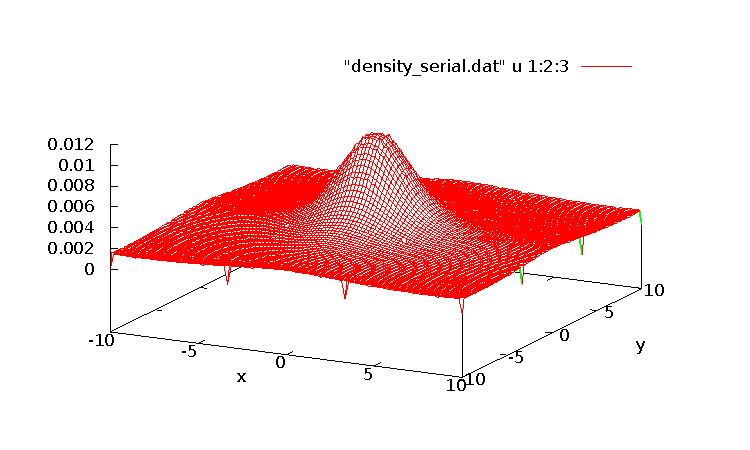
\includegraphics[width=\textwidth, keepaspectratio]{diffusion.pdf}
\end{center}

The code for the parallelization is given by:\\

\begin{lstlisting}[language=CodeBlocks]
 52 #pragma omp parallel for collapse(2)        
 53         for(size_type i = 0; i < N_; ++i) {
 54             for(size_type j = 0; j < N_; ++j) {
 55                 rho_tmp[i*N_ + j] = rho_[i*N_ + j] +
 56                 fac_
 57                 *
 58                 (
 59                  (j == N_-1 ? 0. : rho_[i*N_ + (j+1)])
 60                  +
 61                  (j == 0    ? 0. : rho_[i*N_ + (j-1)])
 62                  +
 63                  (i == N_-1 ? 0. : rho_[(i+1)*N_ + j])
 64                  +
 65                  (i == 0    ? 0. : rho_[(i-1)*N_ + j])
 66                  -
 67                  4.*rho_[i*N_ + j]
 68                  );
 69             }
 70         }
 71         /// use swap instead of rho_=rho_tmp. this is much more efficient, because it does not have to copy
 72         /// element by element.
 73 
 74 #pragma omp barrier
 75 #pragma omp master
 76         using std::swap;
 77         swap(rho_tmp, rho_);
\end{lstlisting}


The scaling behaviour resulted in the following plots: \\
\begin{minipage}[!t]{0.5\textwidth}
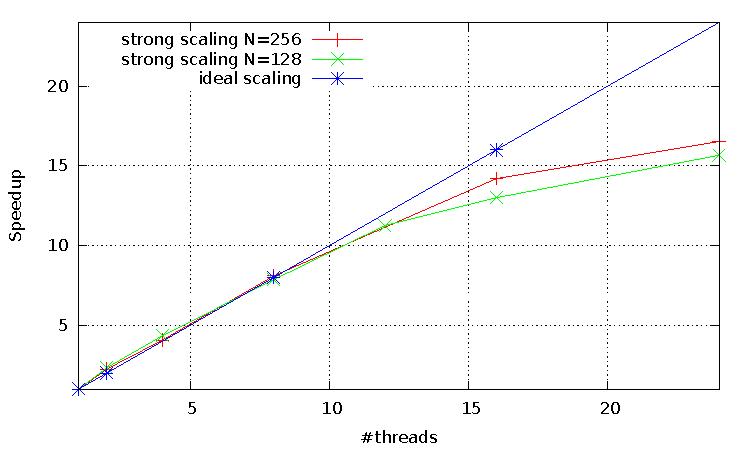
\includegraphics[width=\textwidth, keepaspectratio]{strong_scaling.pdf}
\end{minipage}
\begin{minipage}[!t]{0.5	\textwidth}
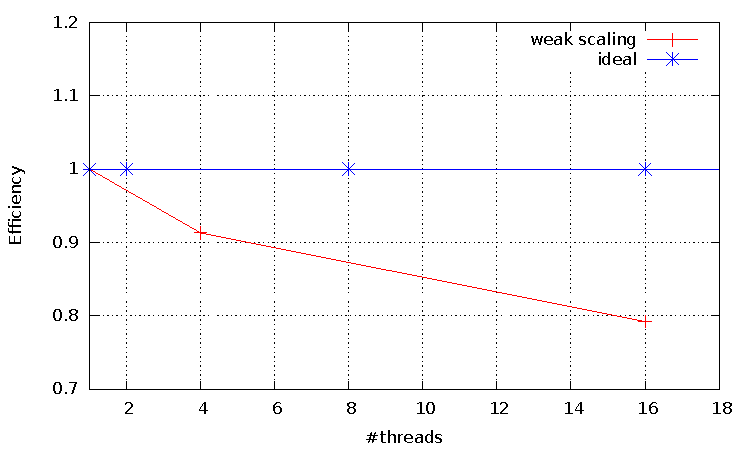
\includegraphics[width=\textwidth]{weak_scaling.pdf}
\end{minipage}

The total amount of heat and the cloud resulted in the following plots. Interestingly just a plot for a short time ($\delta t= 0.001$) with $128$ steps brought a reasonable result for these quantities. For all other trials the results seemed similar to the second graph. Also changing the diffusion constant did not alter this outcome. We expect an error in the simulation. The method used was monte carlo integration (as in the code below).
\begin{lstlisting}[language=CodeBlocks]
 94     value_type mc_rho()
 95     {
 96             size_type mc_steps2_=0;
 97             value_type mc_result2_=0, mc_sum2_=0;
 98 
 99             while(mc_steps2_ < 10000)
100             {
101                     mc_sum2_+=rho_[(rand()%N_)*N_ + (rand()%N_)];
102                     mc_steps2_++;
103             }
104             mc_result2_ = L_*mc_sum2_/10000.;
105             return (mc_result2_);
106     }
\end{lstlisting}

\begin{minipage}[!t]{0.45\textwidth}
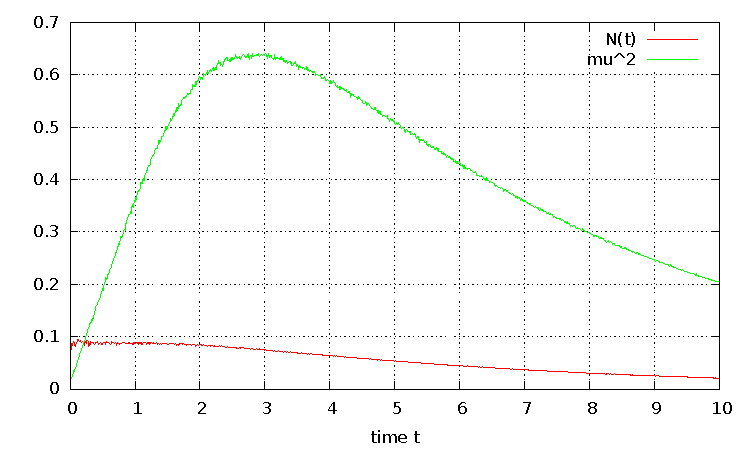
\includegraphics[width=\textwidth, keepaspectratio]{rho_evolution.pdf}
\end{minipage}
\begin{minipage}[!t]{0.45\textwidth}
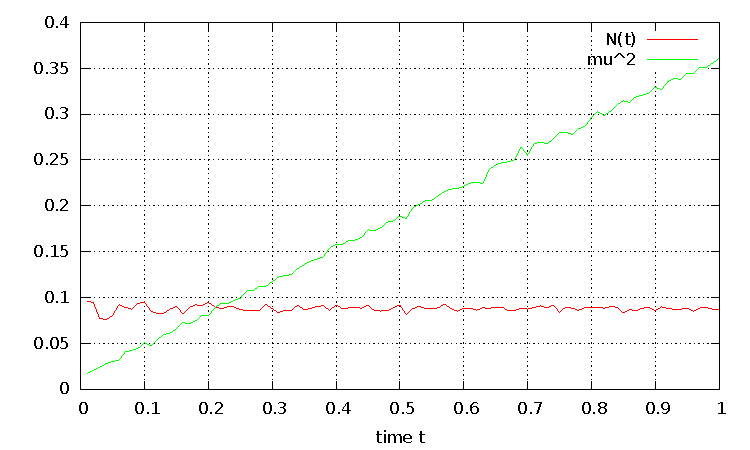
\includegraphics[width=\textwidth]{rho_evolution_high_time.pdf}
\end{minipage}


\subsection{Appendix}
In the following i append the source code of some of the tasks:\\
\begin{lstlisting}[language=CodeBlocks]
  1 // CODE BASED ON THE LECTURE (solution) CODE FROM HPCSE-I, ETHZ
  2 // CHANGES ARE ACCORDINGLY JUST DONE BY THE PARALLELIZATION 
  3 // OF USING OPEN MP
  4 // Leonard Wossnig, 14.10.14
  5 // compile and link using:
  6 // g++ -fopenmp <codename>.cXX
  7 // using #pragram omp parallel 
  8 
  9 
 10 #include <iostream>
 11 #include <algorithm>
 12 #include <string>
 13 #include <fstream>
 14 #include <cassert>
 15 #include <vector>
 16 #include <cmath>
 17 #include <omp.h>
 18 #include <thread>
 19 #include <cstdlib>
 20 #include "timer.cpp"
 21 
 22 
 23 typedef double value_type;
 24 typedef std::size_t size_type;
 25 
 26 class Diffusion2D {
 27 
 28 public:
 29     Diffusion2D(const value_type D, //Diffusion constant
 30                 const value_type L, // length of interval
 31                 const size_type N,  //steps of grid (1d)
 32                 const value_type dt) //timestep
 33     : D_(D), L_(L), N_(N), Ntot(N_*N_), dt_(dt)
 34     {
 35         /// real space grid spacing
 36         dr_ = L_ / (N_ - 1);
 37 
 38         /// stencil factor
 39         fac_ = dt_ * D_ / (dr_ * dr_);
 40 
 41         rho_.resize(Ntot, 0.);
 42         rho_tmp.resize(Ntot, 0.);
 43 
 44         initialize_density();
 45 
 46     }
 47 
 48     void advance()
 49     {
 50         /// Dirichlet boundaries; central differences in space, forward Euler
 51         /// in time
 52 #pragma omp parallel for collapse(2)        
 53         for(size_type i = 0; i < N_; ++i) {
 54             for(size_type j = 0; j < N_; ++j) {
 55                 rho_tmp[i*N_ + j] = rho_[i*N_ + j] +
 56                 fac_
 57                 *
 58                 (
 59                  (j == N_-1 ? 0. : rho_[i*N_ + (j+1)])
 60                  +
 61                  (j == 0    ? 0. : rho_[i*N_ + (j-1)])
 62                  +
 63                  (i == N_-1 ? 0. : rho_[(i+1)*N_ + j])
 64                  +
 65                  (i == 0    ? 0. : rho_[(i-1)*N_ + j])
 66                  -
 67                  4.*rho_[i*N_ + j]
 68                  );
 69             }
 70         }
 71         /// use swap instead of rho_=rho_tmp. this is much more efficient, because it does not have to copy
 72         /// element by element.
 73 
 74 #pragma omp barrier
 75 #pragma omp master
 76         using std::swap;
 77         swap(rho_tmp, rho_);
 78 //#pragma omp flush 
 79     }
 80 
 81     void write_density(std::string const& filename) const
 82     {
 83         std::ofstream out_file(filename, std::ios::out);
 84 
 85         for(size_type i = 0; i < N_; ++i) {
 86             for(size_type j = 0; j < N_; ++j)
 87                 out_file << (i*dr_ - L_/2.) << '\t' << (j*dr_ - L_/2.) << '\t' << rho_[i*N_ + j] << "\n";
 88             out_file << "\n";
 89         }
 90         out_file.close();
 91     }
 92 
 93 
 94     value_type mc_rho()
 95     {
 96             size_type mc_steps2_=0;
 97             value_type mc_result2_=0, mc_sum2_=0;
 98 
 99             while(mc_steps2_ < 10000)
100             {
101                     mc_sum2_+=rho_[(rand()%N_)*N_ + (rand()%N_)];
102                     mc_steps2_++;
103             }
104             mc_result2_ = L_*mc_sum2_/10000.;
105             return (mc_result2_);
106     }
107 
108 
109     value_type mc_cloud()
110     {
111             size_type mc_steps_=0;
112             value_type mc_result_=0, mc_sum_=0;
113 
114             size_type j=0;
115             size_type i=0;
116             while(mc_steps_ < 10000)
117             {
118                     j = (rand()%N_); //really bad rng but quick implementation for now
119                     i = (rand()%N_); // -"-
120                     mc_sum_ += rho_[i*N_+j]*((i*dr_ - L_/2.)*(i*dr_ - L_/2.) + (j*dr_ - L_/2.)*(j*dr_ - L_/2.)) ;
121                     mc_steps_++;
122             }
123             mc_result_ = L_*mc_sum_/10000.;
124             return (mc_result_);
125     }
126 
127 private:
128 
129     void initialize_density()
130     {
131         /// initialize rho(x,y,t=0)
132         value_type bound = 1/2.;
133 
134         for (size_type i = 0; i < N_; ++i) {
135             for (size_type j = 0; j < N_; ++j) {
136                 if (std::abs(i*dr_ - L_/2.) < bound && std::abs(j*dr_ - L_/2.) < bound) {
137                     rho_[i*N_ + j] = 1;
138                 } else {
139                     rho_[i*N_ + j] = 0;
140                 }
141             }
142         }
143         std::cout << "Initialized density, now running programm with " << std::thread::hardware_concurrency() <<" concurrent supported threads in parallel.\n";
144 #pragma omp parallel
145 #pragma omp critical (output) 
146         std::cout << "Thread " << omp_get_thread_num() << " of " << omp_get_num_threads() << " threads." << std::endl;
147 
148     }
149 
150     value_type D_, L_;
151     size_type N_, Ntot;
152 
153     value_type dr_, dt_, fac_;
154 // MC variables
155 
156     std::vector<value_type> rho_, rho_tmp;
157 };
158 
159 
160 int main(int argc, char* argv[])
161 {
162     std::ofstream out("rho_evolution.txt");
163     if (argc < 5) {
164         std::cerr << "Usage: " << argv[0] << " D L N dt" << std::endl;
165         return 1;
166     }
167 
168     const value_type D  = std::stod(argv[1]);
169     const value_type L  = std::stod(argv[2]);
170     const size_type  N  = std::stoul(argv[3]);
171     const value_type dt = std::stod(argv[4]);
172 
173 
174     Diffusion2D system(D, L, N, dt);
175     system.write_density("density.0.dat");
176 
177     srand(time(NULL));
178 
179     const value_type tmax = 10000 * dt;
180     value_type time = 0;
181     int w_count= 0;
182     Timer t;
183     t.start();
184 
185     while(time < tmax){
186         system.advance();
187         w_count++;
188         if(w_count%100==0){
189           out << time << "    " << system.mc_rho() << "   " << system.mc_cloud() <<std::endl;
190         }
191         time += dt;
192     }
193 
194     t.stop();
195 
196     std::cout << "Timing : " << N << " " << t.duration() << std::endl;
197 
198     system.write_density("density_serial.dat");
199 
200     out.close();
201     return 0;
202 }
\end{lstlisting}
\end{document}